%
% Slide template for the FreeBSD Developer Summit.
% Take it or leave it :-)
%
% It requires LaTeX and LaTeX Beamer [1] to compile.
% pdfLaTeX is recommended for compilation as it produces
% PDF file immediately.
%
% $ pdflatex some.latex
%
%
% It is also recommended to convert images to PDF
% by using ImageMagick ("convert") before including them.
%
% [1] http://latex-beamer.sourceforge.net
%

\documentclass{beamer}

\usepackage{url}
\usepackage[english]{babel}
\usepackage{verbatim}
\usepackage{graphicx}
\usepackage{listings}

\mode<presentation>
{
  \definecolor{beamer@gker}{rgb}{0.8,0.0,0.0}
  \setbeamercolor*{structure}{fg=beamer@gker}
  \logo{
\includegraphics[scale=0.5]{logo.pdf}}
}

\setbeamertemplate{footline}[text line]{%
  \parbox{\linewidth}{\vspace*{-8pt}
  some text
  \hfill
  \insertshortauthor
  \hfill
  \insertframenumber\ of \inserttotalframenumber}}
\setbeamertemplate{navigation symbols}{}

\title{FreeBSD package management system}
\author{Vsevolod Stakhov \\ \url{vsevolod@FreeBSD.org}}
\institute{
\includegraphics[scale=0.5]{logo.pdf}}
\date{ruBSD conference \
December 14, 2013}

\begin{document}

\begin{frame}[plain]
  \titlepage
\end{frame}

\begin{frame}
\frametitle{Ports and packages}
Ports is the comprehensive system of source packages.
\begin{itemize}
  \item Mature.
  \item Clear and well defined.
  \item Simple (sometimes not).
\end{itemize}
\end{frame}

\begin{frame}[fragile]
\frametitle{Ports before pkg}
\begin{figure}[h!]
  \centering
  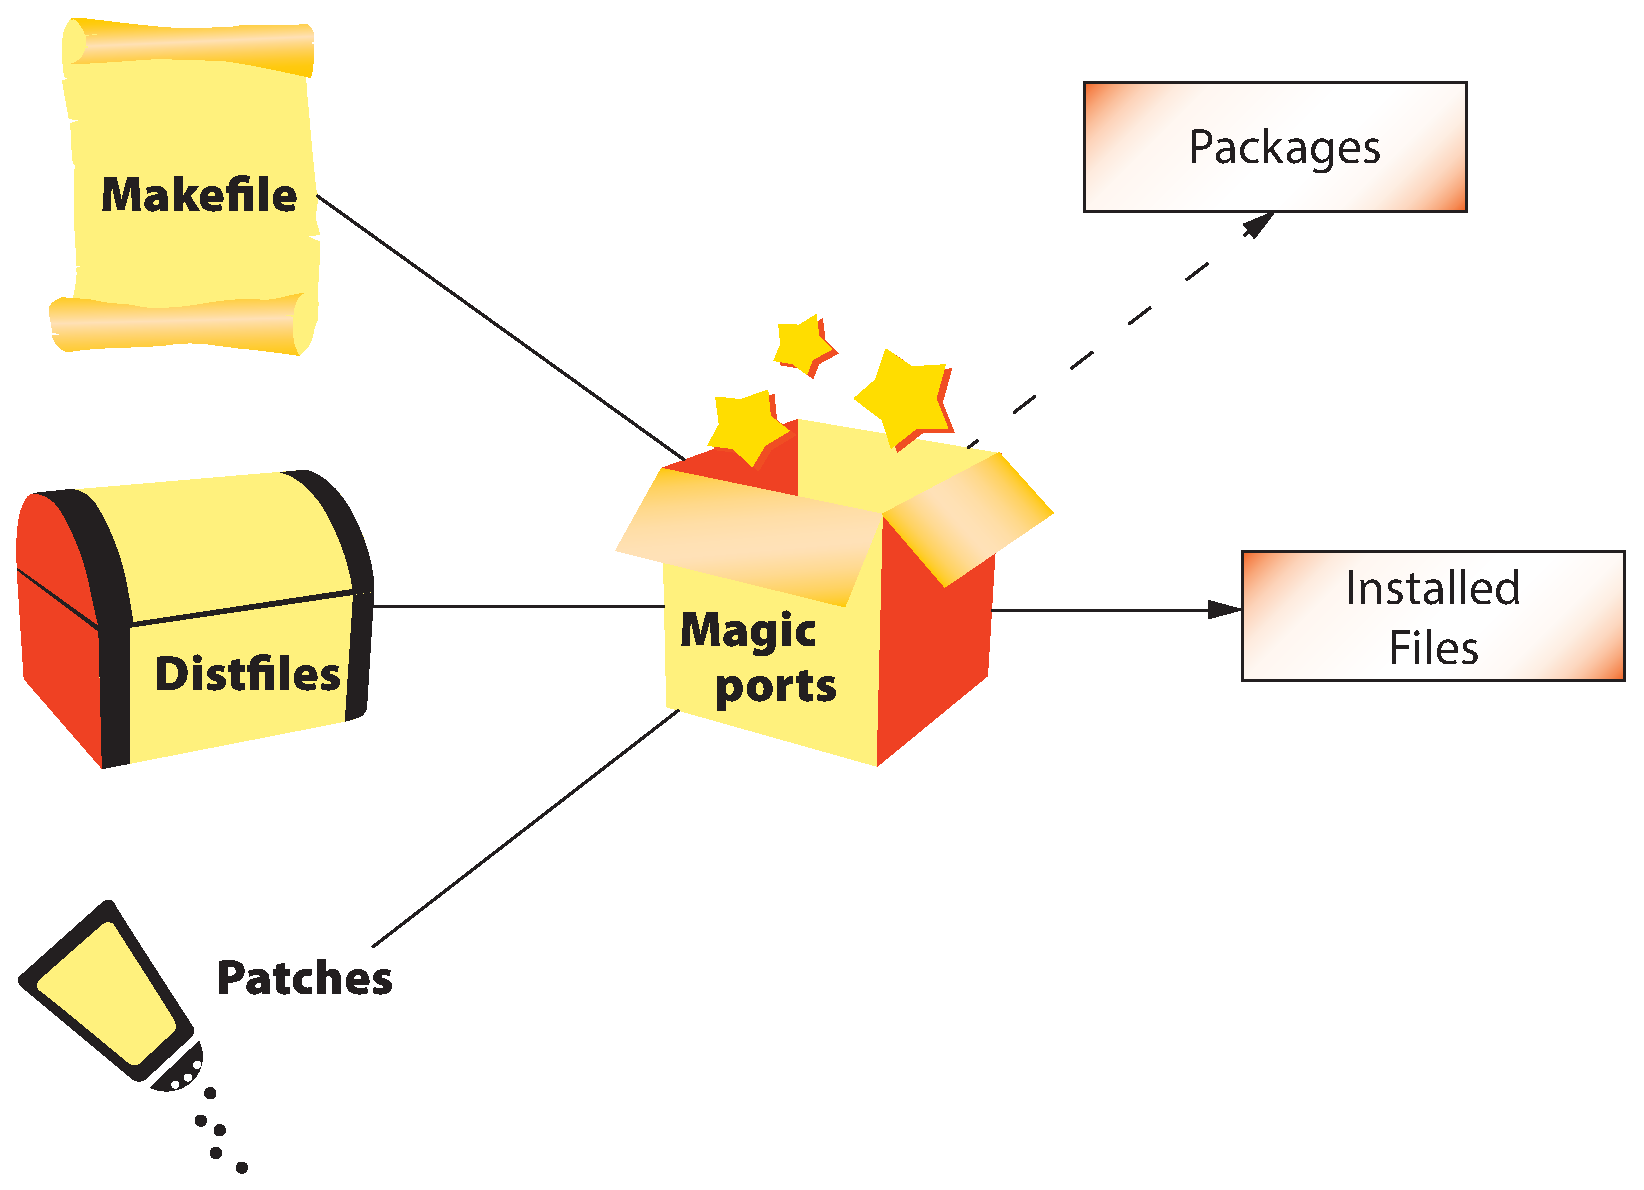
\includegraphics[width=0.95\textwidth]{q1.eps}
\end{figure}
\end{frame}

\begin{frame}
\frametitle{Planned ports and pkg interaction}
\begin{figure}[h!]
  \centering
  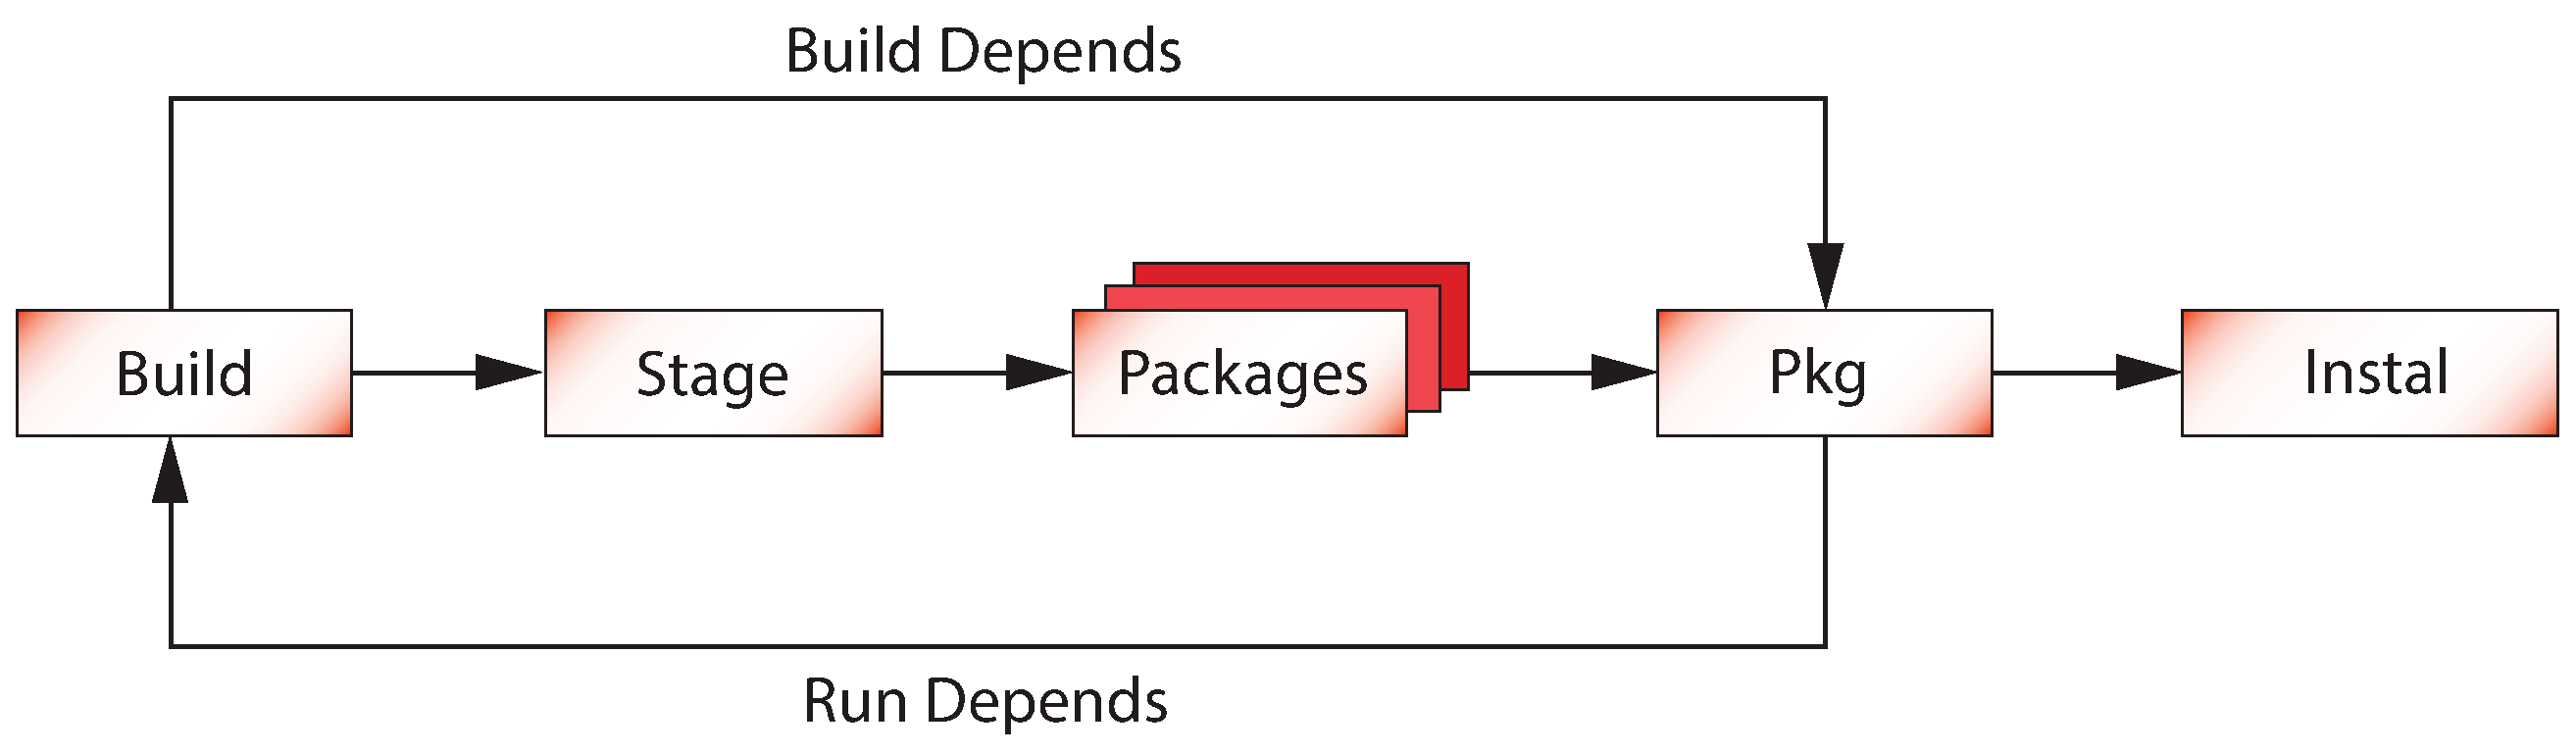
\includegraphics[width=0.95\textwidth]{q2.eps}
\end{figure}
\end{frame}

\begin{frame}
\frametitle{Ports and packages}
\begin{itemize}
  \item Ports are used to build packages.
  \item Dependencies are resolved by pkg, not make.
  \item Stable branch of ports has an appropriate stable branch of packages.
  \item Encourage users to install software from binary packages.
  \item But do not prevent them from building custom packages from the ports.
\end{itemize} 
\end{frame}

\begin{frame}
\frametitle{Pkg architecture}
%% Picture 3
\end{frame}

\begin{frame}
\frametitle{Pkg internals}
%% Picture 4
\end{frame}

\begin{frame}
\frametitle{The current problems with pkg}
\begin{itemize}
  \item Legacy ports support (with no staging, for example).
  \item Plain dependencies style.
  \item Immature codebase.
  \item Naive solver.
\end{itemize}
\end{frame}

\begin{frame}
\frametitle{The problems of the solver in pkg}

\begin{itemize}
\item Absence of conflicts resolving/handling;
\item No alternatives support;
\item Can perform merely a single task: install, upgrade, remove or autoremove,
so install task cannot remove packages for examle.
\end{itemize}

\end{frame}


\begin{frame}
\frametitle{The existing work}

There are many examples of solvers, for example:
\begin{itemize}
  \item \texttt{libsolv} - the complete solver and package management library;
  \item \texttt{Apt} solvers interface;
  \item \texttt{Mancoosi} - a European research project that compares and study
  different solvers;
\end{itemize}

\end{frame}

\begin{frame}[fragile]
\frametitle{External solvers}
To interact with an external solver we have chosen CUDF format used in the
Mancoosi project:
\bigskip
{\tiny
	\begin{verbatim}
	package: devel/libblah
	version: 1
	depends: x11/libfoo

	package: security/blah
	version: 2
	depends: devel/libblah
	conflicts: security/blah-devel
	
	\end{verbatim}
}
\end{frame}

\begin{frame}
\frametitle{How to implement a solver}

Alternatives:
\begin{itemize}
  \item Write own logic of dependencies and conflicts resolution?
  \pause
  \item Use some existing solution?
  \pause
  \item Use some known algorithm?
  \pause
\end{itemize}
\bigskip
{\large SAT solver}
\bigskip
$(x_1 \| \neg x_2 \| x_3) \& (x_3 \| \neg x_1) \& (x_2)$
\end{frame}

\begin{frame}
\frametitle{Making a SAT problem}
\begin{itemize}
  \item Assign a variable to each package: 
  package A $\to a_1$, package B $\to a_2$
  \item Interpret a request as a set of unary clauses:
  \begin{itemize}
    \item Install/Upgrade package A $\to (a_1)$
    \item Delete package B $\to (\neg a_2)$
  \end{itemize}
  \item Convert dependencies and conflicts to disjuncted clauses
\end{itemize}

\end{frame}

\begin{frame}
\frametitle{Converting dependencies and conflicts}
\begin{itemize}
  \item If we have a dependency for package A from package B that is provided by
packages $B_1$ and $B_2$ (which may be different versions of the same package),
then we can either have package A not installed or any of B installed:
  \bigskip
$(\neg A \| B_1 \| B_2)$
  \item If we have a conflict between versions of B ($B_1$, $B_2$ and $B_3$)
 then we must claim that merely a single version can be installed:
  \bigskip
$(\neg B_1 \| \neg B_2) \& (\neg B_1 \| \neg B_3) \& (\neg B_2 \| \neg
B_3)$
\end{itemize}
\end{frame}

\begin{frame}
\frametitle{The solving of SAT problem}

The SAT problem itself is NP complete and assume the full depth search. Luckily
there are common tricks to reduce the problem complexity by skipping some paths.
Moreover, for packages we assume to avoid deinstall packages till they are not
in conflict with the requested ones.
\begin{itemize}
  \item Trivial propagation - solve unary clauses;
  \item Unit propagation - solve clauses with only a single unsolved variable;
  \item Conflicts learning - if we assign some free variable and detect a
  conflict during unit propagation, we can fallback and learn that this variable
  must be inversed;
\end{itemize}
\end{frame}

\begin{frame}
\frametitle{Solvers and PkgNG}

For PkgNG we need to adopt the current jobs handling structure to support SAT
solver and external solvers. The following steps are done:
\begin{itemize}
  \item A request is splitted to install/upgrade and delete requests which
  could be passed simultaneously to the solver;
  \item A conflicts between packages are detected with a repository creation;
  \item All depends, reverse and conflicts of the requested packages are
  analyzed and the package universe is created;
  \item Each package is defined by its origin and the digest of significant
  fields (version, options and so on);
\end{itemize}
\end{frame}

\begin{frame}
\frametitle{Solvers and PkgNG}
\begin{itemize}
  \item After the universe and the request are formed it is possible to pass them to an
external solver using CUDF exporter or to the internal SAT solver by creating a
SAT problem corresponding to this package task.
  \item After solving our request pkgng will be able to install required and
delete conflicting packages. Upgrade procedure can be the same: we remove the old
version of package and install a new one.
\end{itemize}
\end{frame}

\begin{frame}
\frametitle{Perspectives}

\begin{itemize}
  \item Using pkg solver for ports management (need to think how to form
  universe from the ports).
  \item New dependencies and conflicts: not just from a plain package but from
  specific versions or variants (such as $libblah > 1.0 +option_1, +option_2 \|
  libfoo != 1.1$).
  \item Better support of multiple repositories (counting that they have shared
  conflicts).
  \item Provides and alternatives (support from the ports is badly required).
  \item We can test various of experimental external solvers and eventually
  select the best one.
\end{itemize}
\end{frame}

\begin{frame}
\frametitle{Project Status}
\begin{itemize}
  \item Currently, the new solver is very near for initial testing status.
  \item The other big task is to adopt ports to the new pkg features and
  integrate pkgng more deeply to the ports infrastructure, for example for dependencies resolution and
install/upgrade/delete tasks solving.
  \item Eventually we need to improve dependencies and conflicts from the plain
  structure to the advanced dependency formulas.
\end{itemize} 
\end{frame}

\begin{frame}
\begin{center}

\includegraphics{logo.pdf}
{\Large Thank you for your attention!} \\
\emph{ask questions}
\end{center}
\end{frame}

\end{document}
